\documentclass[a4paper,12pt,twoside]{article}
\usepackage{mypackage}

\begin{document}
 \section{Calculating the mean temperatures of every day of the year}
 \label{sec:3.2}
 How does the temperature change over the course of a year? Recording the temperature
 every day for one year might give some indication, but leaves a large margin of error.
 With a dataset stretching almost three hundred years we can calculate the mean
 temperature of each day and get a much more reliable result.
 
 The mean temperature of a certain day is the sum of the temperatures recorded at
 that day, divided by the number of days it has been recorded:
 \begin{equation}
  \label{eq:MeanTempPerDay}
  \overline{T(day 1)} = \frac{T(day 1, year 1)+T(day 1, year 2)+...+T(day 1, year N)}{N}
 \end{equation} 
  
 
 Reading from the datafile, each datatype was put in a vector (excluding the year
 1722 since we don't have all the data for that year, and the 29th of february for
 simplicity). We now have the data in vectors of equal length $(2013-1722)\times(365)=106215$,
 where the data in the same position in the vectors correlate.
 
 Next, the data needed to be separated according to which year it belonged. An empty
 vector of length 365 was created, and then (using a for-loop) the temperature belonging
 to day $k$ was added to the $(k-1)$:th position in the vector. The number of times this
 summation happened was also recorded (it should be equal to the number of years, $291$).
 
 \begin{verbatim}
  	//loop for calculating the mean temperatures of each day
	for (UInt_t k=0; k < vyear.size(); k++){
	
	...
	
	if (vyear.at(k) != vyear.at(k+1)){
		daycounter = 365;
	  }

	else if (vyear.at(k) == vyear.at(k+1)){
	  daycounter = daycounter+1;
	  }
	
	sumtempvec.at(daycounter-1)
	          =sumtempvec.at(daycounter-1) + vtemp.at(k);
	
	...
	
	if (daycounter == 365){
	  daycounter = 0;
	  yr_it = yr_it +1; //the number of years we've iterated over
	  }
	}
 \end{verbatim}
 Using another for-loop to divide each element of the vector with the number of years,
 we now had a vector where each element was the mean temperature of the day
 corresponding to the element's position.
 \newline
 The standard deviation is defined as 
  \begin{equation}
 \label{eq:StdDev}
 \sigma = \sqrt{\frac{\sum\limits_{i=1}^{n} (t_{i}-\bar{t})^2}{n-1}}
 \end{equation}
 
 The mean temperature of each day $\bar{t}$ had been calculated as above, and now another 
 empty vector of length 365 was created. In the same way as before, we looped over the vectors
 containing the data, this time putting the square of the sum of the differences between the
 temperature of the current iteration and the mean temperature of the current day in the vector:
 
 \begin{verbatim}
    	...
  	vStdDev.at(daycounter-1) +=
  	    (vtemp.at(k)-sumtempvec.at(daycounter-1))*
  	    (vtemp.at(k)-sumtempvec.at(daycounter-1));
  	...
 \end{verbatim}

 
 After the iteration we therefore had ${\sum\limits_{i=1}^{n} (t_i - \bar{t})}^2$. Using another for-loop, each element in the vector
 was then divided by the number of years ($n$) in the same way as before and the square root of these values was
 calculated, to get the standard deviation for each day of the year.
 
 \begin{verbatim}
	for (UInt_t q=0;q<vStdDev.size();q++){
	  vStdDev.at(q) = TMath::Sqrt(vStdDev.at(q)/(yr_it-1));
	}
 \end{verbatim}
 
 Finally we had two vectos, one containing the mean temperatures of each day, and the other
 containing the standard deviation, where the position in the vector correlated to the day
 of a year. Using yet another for-loop, the elements in the two vectors were set to be the
 bin content and the bin errors in a histogram. This produced the histogram shown in
 figure \ref{fig:tempPerDay}.
 
 \begin{figure}[htb]
  \begin{center}
   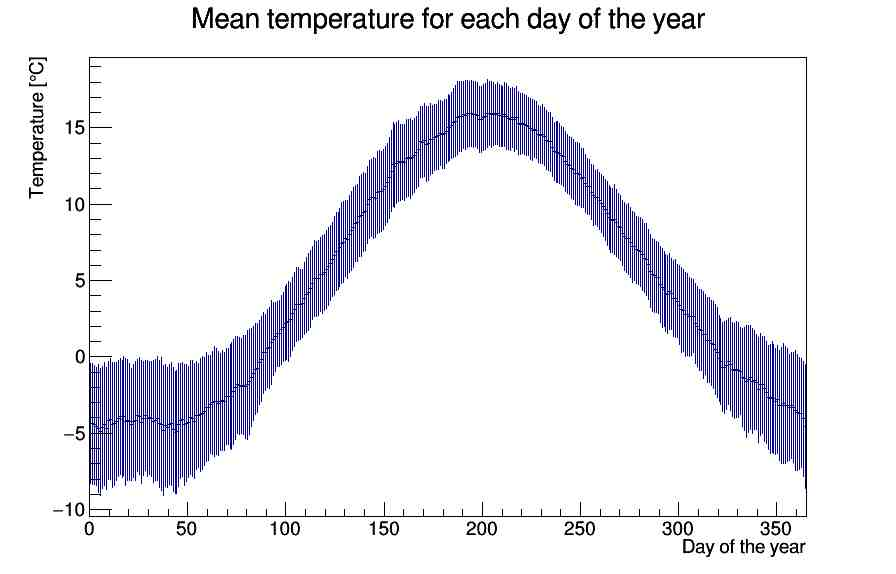
\includegraphics[width=13cm]{../Code/tempPerDay.jpg}
   \caption{Histogram showing the mean temperature of every day of the year}
   \label{fig:tempPerDay}
  \end{center}
 \end{figure}
 
 From the histogram we can see that the temperature is at its peak around day 200, that is July 19, and
 not surprisingly it is coldest around New Years and the beginning of the year. The mean temperature remains
 approximately constant at around $-4 ^{\circ}$C until day 50 (February 19), when it begins to rise and crosses into
 positive temperatures around day 95 (April 5). However, the error bars showing deviations from the mean allow for a large
 variation of temperature of approximately $15 ^{\circ}$C in the beginning of the year (this decreases to approximately $5 ^{\circ}$C
 later on), showing that the temperatures during springtime can vary greatly from year to year.
 
 
\end{document}



